\chapter{Analisis}
\label{chap:analisis}

Pada bab ini dijelaskan mengenai analisis pengiriman data dari node sensor ke base station pada WSN, analisis terhadap protokol transfer yang \textit{reliable} pada \textit{Wireless Sensor Network} untuk digunakan dalam membangun aplikasi transfer data, dan analisis aplikasi pengiriman data pada WSN.

\section{Analisis Proses Pengiriman Data Dari Node Sensor Ke Base Station Pada WSN}
Pengiriman data pada WSN dibagi menjadi dua yaitu pengiriman data dari base station ke setiap node sensor (downstream) dan pengiriman data dari setiap node sensor ke base station (upstream). Pengiriman downstream biasanya adalah perintah yang diberikan oleh base station kepada node sensor, sedangkan pengiriman upstream adalah pengiriman data hasil sensing setiap node sensor kepada base station. Dalam melakukan pengiriman ini dapat dilakukan dengan single hop atau multi hop tergantung pada komunikasi yang digunakan. 

Pengiriman data hasil sensing dari node sensor ke base station sendiri dapat dilakukan dengan dua cara yaitu setiap data hasil sensing langsung dikirimkan ke base station tanpa melalui proses apapun pada node sensor dan data hasil sensing diproses dahulu pada node sensor lalu dikirimkan. Kedua cara ini sebenarnya dapat digunakan sesuai dengan kebutuhkan dan kapasitas penyimpanan pada node sensor. Node sensor memiliki tempat penyimpanan yang kecil, sehingga kode program yang dibuat juga tidak dapat terlalu besar. 

Pada skripsi ini digunakan cara dengan mengirim langsung data mentah yang didapat dari node sensor tersebut. Penulis memilih cara ini karena penyimpanan node sensor yang kecil. Selain itu untuk diimplementasi cara ini lebih mudah dibandingkan dengan melakukan memprosesan terlebih dahulu. Karena tujuan utama pada skripsi ini adalah membangun aplikasi untuk transfer data maka pada base station hanya memerlukan data mentah.

\section{Analisis Terhadap Protokol Transfer Yang Reliable Pada WSN Untuk Digunakan Dalam Membangun Aplikasi Transfer Data}
Tidak semua protokol pengiriman data pada WSN mendukung pengiriman data yang \textit{reliable}. Pada WSN terdapat beberapa protokol yang mendukung pengiriman data reliable. Untuk memastikan data yang reliable ini dilakukanlah pengiriman ulang (retransmission) data yang hilang atau \textit{loss}. Data yang dikirim ulang ini dapat berasal dari hasil \textit{sensing} node sensor atau data dari base station seperti perintah atau \textit{method} untuk melakukan sesuatu. Pada skripsi ini data yang dikirim ulang adalah data hasil \textit{sensing} sehingga protokol yang digunakan adalah protokol dengan arah pengiriman \textit{upstream}. Setiap protokol memiliki spesifikasi yang berbeda-beda pada arah \textit{retransmission}, data yang dikirim, mekanisme dan \textit{acknowledge} yang digunakan. 

Pada skripsi ini dibangun aplikasi transfer data pada WSN. Aplikasi yang dibangun ini juga menangani pengiriman data yang \textit{reliable}. Pengiriman data yang terjadi adalah pengiriman data dari setiap node sensor hingga sampai ke base station (\textit{upstream}). Data yang didapat oleh node sensor ini dapat diteruskan ke node tetangganya dahulu sebelu sampai ke tujuan akhir yaitu \textit{base station}. Berdasarkan Tabel~\ref{tab:protokol_reliable} terdapat beberapa protokol yang diadaptasi untuk membuat aplikasi transfer data ini. 

Aplikasi transfer data yang dibuat ini akan menangani data yang loss menggunakan mekanisme hop-by-hop dengan bantuan ACK dalam memastikan data sampai ke node tetangganya. Dengan mekanisme hop-by-hop akan lebih cepat untuk mengirimkan ulang data yang loss. Jika dibandingkan dengan mekanisme end-to-end retransmission maka reliabilitas data akan diperiksa oleh base station. Jika base station menemukan ada data yang loss, maka base station akan meminta node sensor untuk mengirimkan ulang data yang loss tersebut. Namum permasalahan pada mekanisme end-to-end adalah jika arsitektur yang dibangun adalah multi hop maka base station akan meminta node yang terhubung dengan base station meneruskan pesan ke node sensor tetangganya hingga ke node sensor yang melakukan \textit{sensing} untuk mengirim ulang data. 

Dengan mekanisme hop-by-hop, saat salah satu node mengirimkan data ke node tetangganya, node pengirim akan menunggu ACK dari node penerima. Saat menunggu ACK dari node tetangganya ini digunakan juga mekanisme \textit{timer-driven}. Dengan menggunakan mekanisme \textit{timer-driven} ini, waktu menunggu ACK dapat dibatasi. Jika sudah melewati batas waktu menunggu ACK tersebut, maka data akan dianggap tidak diterima oleh penerima dan pengirim akan mengirimkan ulang data. Saat melakukan pengiriman ulang data ini bisa saja terjadi pengulangan data yang diterima. Jika ini terjadi maka digunakan \textit{sequence number} untuk memastikan urutan data.

%class diagram
\section{Analisis Aplikasi Pengiriman Data Pada WSN}
Pada skripsi ini dibuat aplikasi yang dapat melakukan transfer data dari node sensor ke base station. Aplikasi ini digunakan untuk mengetahui keadaan suatu tempat atau daerah dengan bantuan node sensor untuk melakukan mendapatkan data (sensing). Aplikasi ini memiliki beberapa fungsi. Fungsi utama pada aplikasi ini adalah untuk melakukan transfer data dari setiap node sensor. Fungsi lain pada aplikasi ini dijelaskan menggunakan diagram \textit{use case} pada Gambar~\ref{fig:usecase} dan skenario pada Tabel~\ref{tab:skenario1} sampai Tabel~\ref{tab:skenario3}.

\begin{figure}[htbp]
	\centering
	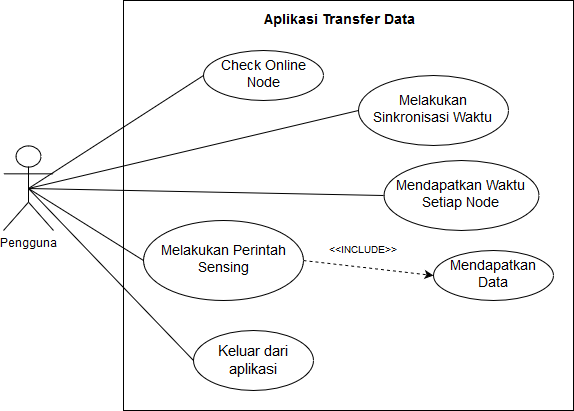
\includegraphics[scale=0.6]{usecase}
	\caption{Diagram \textit{use case} aplikasi data transfer pada WSN}
	\label{fig:usecase}
\end{figure}

\begin{table}[htbp]
    \centering
    \begin{tabular}{|p{3cm}|p{10cm}|}
    \hline
        Nama & Melakukan sinkronisasi waktu\\
    \hline
    \hline
        Deskripsi & Melakukan sinkronisasi waktu untuk mengetahui kapan data dikirim dari node sensor dan diterima oleh base station. \\
    \hline
        Aktor & Pengguna \\
    \hline
        Pre-kondisi & Aplikasi dimulai \\
    \hline
        Alur Skenario Utama & 
        \begin{enumerate}
            \item Sistem memuat aplikasi.
            \item Sistem menampilkan menu untuk dipilih pengguna.
            \item Pengguna memilih menu sinkronisasi waktu.
            \item Sistem melakukan sinkronisasi waktu pada setiap node sensor.
            \item Sistem menampilkan menu.
        \end{enumerate}\\
    \hline
    \end{tabular}
    \caption{Tabel skenario melakukan sinkronisasi waktu.}
    \label{tab:skenario1}
\end{table}

\begin{table}[htbp]
    \centering
    \begin{tabular}{|p{3cm}|p{10cm}|}
    \hline
        Nama & Menjalankan fungsi untuk \textit{sensing}\\
    \hline
    \hline
        Deskripsi & Pengguna menjalankan fungsi ini untuk membuat node sensor melakukan sensing dan mengirimkan data.\\
    \hline
        Aktor & Pengguna \\
    \hline
        Pre-kondisi & Sudah dilakukan sinkronisasi waktu pada setiap node sensor\\
    \hline
        Alur Skenario Utama & 
        \begin{enumerate}
            \item Sistem memuat aplikasi.
            \item Sistem menampilkan menu untuk dipilih pengguna.
            \item Pengguna memilih menu untuk \textit{sensing}.
            \item Sistem memerintahkan node sensor untuk melakukan \textit{sensing}.
            \item Sistem mendapatkan data dari setiap node sensor.
        \end{enumerate}\\
    \hline
    \end{tabular}
    \caption{Tabel skenario Menjalankan fungsi untuk \textit{sensing}.}
    \label{tab:skenario2}
\end{table}

\begin{table}[htbp]
    \centering
    \begin{tabular}{|p{3cm}|p{10cm}|}
    \hline
        Nama & Mendapatkan Data\\
    \hline
    \hline
        Deskripsi & Pengguna mendapatkan data hasil \textit{sensing} dari setiap node sensor\\
    \hline
        Aktor & Pengguna \\
    \hline
        Pre-kondisi & Sistem sudah melakukan \textit{sensing} dan data hasil \textit{sensing} sudah didapatkan \\
    \hline
        Alur Skenario Utama & 
        \begin{enumerate}
            \item Sistem memuat aplikasi.
            \item Sistem menampilkan menu untuk dipilih pengguna.
            \item Pengguna memilih menu untuk mendapatkan data.
            \item Sistem mengirimkan data hasil \textit{sensing} kepada pengguna.
        \end{enumerate}\\
    \hline
    \end{tabular}
    \caption{Tabel skenario mendapatkan data.}
    \label{tab:skenario3}
\end{table}

\subsection{Diagram Sequence}
Untuk aplikasi transfer data ini, aliran data dapat dilihat dengan diagram sequence. Diagram sequence dibuat menjadi dua macam sesuai dengan arsitektur yang digunakan yaitu arsitektur flat dengan multi-hop dan arsitektur hierarkikal.

------- Gambar Diagram Seq 1 -------
Keterangan...

------- Gambar Diagram Seq 2 -------
Keterangan...

\subsection{Fitur dan Kebutuhkan Sistem}
Pada skripsi ini aplikasi yang dibangun memiliki fitur utama untuk mengirim data hasil sensing. Sesuai dengan diagram sequence yang dibuat, untuk arsitektur flat dan hierarki terdapat sedikit perbedaan untuk aplikasi yang dibuat. Pada arsitektur flat tidak terdapat cluster head jadi node sensor hanya mengirimkan data ke node tetangganya hingga sampai ke base station, sedangkan pada arsitektur hierarkikal data dikirimkan dahulu ke cluster head sebelum diteruskan ke base station.
...... 
%analisis aplikasinya (fitur) dan kebutuhan sistem (Sistem requirement)
% tentukan untuk yg flat dan hierarki (masing-masing)
